\section{Classifications of Singularities}

\begin{definition}
    We say that a complex-valued function $f$ has an  \textbf{isolated
    singularity} at a point $z=a$ provied there exists an $R>0$ for which  $f$
    is defined and analytic on the punctured ball  $\com{B(a,R)}{\{a\}}$, but
    not on the ball $B(a,R)$. We say that $f$ has a  \textbf{removable
    singularity} at the point $z=a$, if there exists a analytic function
    $g:B(a,R) \xrightarrow{} \C$ such that $g(z)=f(z)$ for all $0<|z-a|<R$.
\end{definition}

\begin{example}\label{example_5.1}
    The functions $\frac{\sin{z}}{z}$, $\frac{1}{z}$, and $\exp{\frac{1}{z}}$
    have isolated singularities at the point $z=0$. However, only
    $\frac{\sin{z}}{z}$ has a removable singularity at $z=0$.
\end{example}

\begin{theorem}\label{5.1.1}
    If a complex-valued function $f$ has an isoloted singularity at a point
    $z=a$, then it is a removable singularity if, and only if
    \begin{equation*}
        \lim_{z \xrightarrow{} a}{(z-a)f(z)}=0
    \end{equation*}
\end{theorem}
\begin{proof}
    Suppose that $f$ is analytic on the annulus $A=\{z \in \C : 0<|z-a|<R\}$
    for some $R>0$. Define  $g(z)=(z-a)f(z)$ for all $z \neq a$, and  $g(a)=0$.
    Suppose also that $\lim{(z-a)f(z)}=0$ as $z \xrightarrow{} a$. Then $g$ is a
    continuous function by definition.

     \begin{figure}[h]
        \centering
        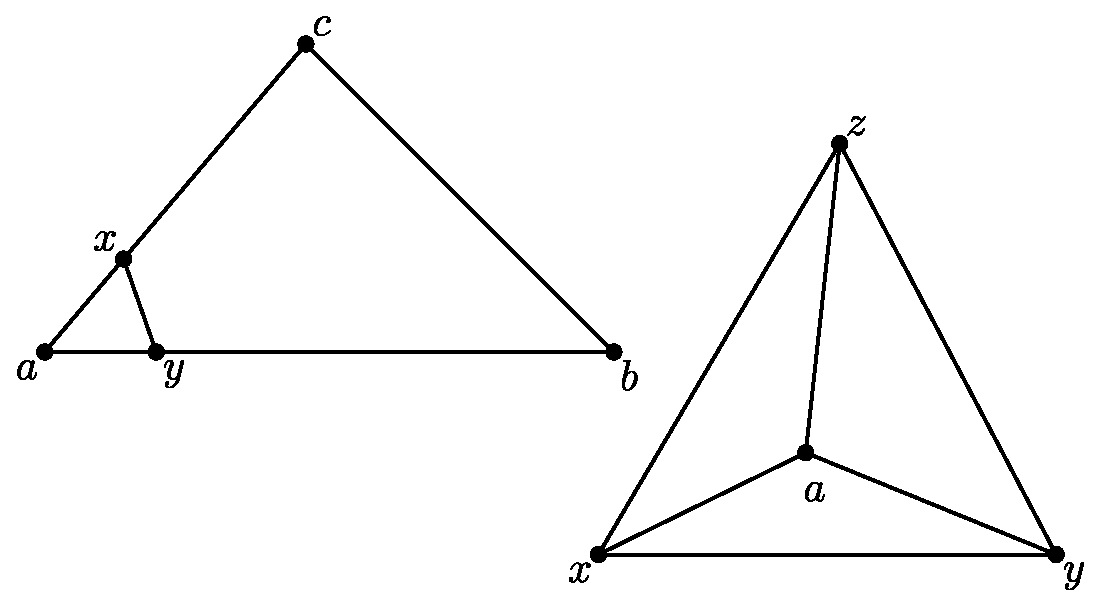
\includegraphics[scale=0.5]{Figures/Chapter5/isolated_sigularities.eps}
        \caption{}
        \label{figure_5.1}
    \end{figure}

    Now, let $T$ be a triangular path in  $B(a,R)$, and let $\Delta$ be the
    interior of $T$, along with the trace of $T$; i.e.  $\Delta=\Int{T} \cup
    \{T\}$. Now, if $a \notin \Delta$, then  $T$ is nullhomotopic, in the
    annulus  $A$, and hence by Cauchy's theorem,  $\int_T{g}=0$. Now, suppose
    that $a$ is a vertex in  $T$, i.e. that  $T=[a,b,c,a]$. Let $x \in [a,c]$
    and $y \in [a,b]$, and let $[x,y]$ the line segment joining $x$ and  $y$
    (see figure \ref{figure_5.1}). Then we form the triangular path
    $T_1=[a,x,y,a]$, and the polygonal path $P=[x,b,c,y,x]$. Then we get
    \begin{equation*}
        \int_T{g}=\int_{T_1}{g}+\int_{P}{g}=\int_{T_1}{g}
    \end{equation*}
    since $\int_P{g}=0$, by Cauchy's theorem (notice that $P$ is nullhomotopic).
    Now, since $g$ is continuous, and  $g(a)=0$, then there is an $\e>0$ for
    which, choosing  $x,y$ such that
    \begin{equation*}
        |g(z)|<\frac{\e}{l} \text{ for all } z \in T_1
    \end{equation*}
    where $l$ is the length of $T$, then we have
    \begin{equation*}
        \Big{|} \int_{T}{g} \Big{|}=\Big{|} \int_{T_1}{g} \Big{|} \leq \e
    \end{equation*}
    This makes $\int_T{g}=0$.

    Now, suppose that $a \in \com{\Delta}{\{T\}}$, and take $T=[x,y,z,x]$ (see
    figure \ref{figure_5.1}). Consider now the triangular paths $T_1=[x,y,a,x]$,
    $T_2=[y,z,a,y]$, and $T_3=[z,x,a,z]$. Now, notice that $\int_{T_j}{g}=0$ for
    all $j=1,2,3$, by similar reasoning to the above argument, we conclude that
     $\int_T{g}=0$. That is, in all cases, by Morera's theorem, $g$ is
     analytic on  $B(a,R)$, since $g(a)=0$, thus $g(z)=f(z)$ for all
     $0<|z-a|<R$, which makes  $a$ a removable singularity.
\end{proof}

\begin{definition}
    If $z=a$ is an isolated singularity of a complex valued function $f$, then
    we call the point $z=a$ a  \textbf{pole} if for every $\e>0$, there is an
    $M>0$ such that
    \begin{equation*}
        |f(z)| \geq M \text{ whenever } 0<|z-a|<\e
    \end{equation*}
    We call the point $z=a$ an \textbf{essential singularity} if it is neither a
    pole, nor a removable singularity.
\end{definition}

\begin{lemma}\label{5.1.2}
    If $U$ is a region of  $\C$, with  $a \in U$, and  $f$ is a analytic
    function on  $\com{U}{\{a\}}$, with a pole at the point $z=a$, then there
    exists a positive integer  $n \im \Z^+$, and a analytic function  $g:U
    \xrightarrow{} \C$ such that
    \begin{equation*}
        g(z)=(z-a)^mf(z)
    \end{equation*}
\end{lemma}
\begin{proof}
    If $f$ has a pole at  $z=a$, then  $\frac{1}{f}$ has a removable singularity
    at $z=a$. Define then  $h(z)=\frac{1}{f(z)}$ for all $z \neq z$, and
    $h(a)=0$. Then $h$ is analytic on the ball  $B(a,R)$, for some $R>0$.
    Now, since  $h(z)=0$, then $h(z)=(z-a)^mh_1(z)$, with some $h_1$ analytic
    and $h_1(a) \neq 0$ for some $m \in \Z^+$. Thus we get
    $(z-a)^mf(z)=\frac{1}{h_1(z)}$. Take, then $g(z)=\frac{1}{h_1(z)}$.
\end{proof}

\begin{definition}
    Let $f$ be a complex-valued function, with a pole at  $z=a$, and let  $m \in
    \Z^+$ be the smallest positive integer for which  $(z-a)^mf(z)$ has a
    removable singularity at $z=a$. Then we call the point $z=a$ a
    \textbf{pole} of \textbf{order} $m$ of  $f$. If $z=a$ is a pole of order
    $1$, we call $z=a$ a \textbf{simple pole}.
\end{definition}

\begin{definition}
    Let $f$ be a complex-valued function with a pole of order  $m$ at  $z=a$ and
    let  $g$ he a complex-valued function such that  $g(z)=(z-a)^mf(z)$, and for
    which $g$ has a power series expansion
    \begin{equation*}
        g(z)=A_m+A_{m-1}(z-a)+\dots+A_1(z-a)^{m-1}+(z-a)^m\sum{a_k(z-a)^k}
    \end{equation*}
    So that
    \begin{equation*}
        f(z)=\frac{A_m}{(z-a)^m}+\dots+\frac{A_1}{(z-a)}+g_1(z)
    \end{equation*}
    with $g_1$ analytic on $B(a,R)$. We call the terms
    \begin{equation*}
        \frac{A_m}{(z-a)^m}+\dots+\frac{A_1}{(z-a)}
    \end{equation*}
    the \textbf{singular part} of $f$ at  $z=a$. We define the  \textbf{Laurent
    series} of $f$ at the point  $z=a$ to be the power series
    \begin{equation*}
        f(z)=\sum_{n=-\infty}^\infty{a_n(z-a)^n}
    \end{equation*}
    We call the series $\sum_{-\infty}^\infty{z_n}$ \textbf{absolutely
    convergent} if both  $\sum_{n=0}^\infty{z_n}$ and
    $\sum_{n=1}^\infty{z {-n}}$ are absolutely convergent. If $u_n$ is a
    function for which $\sum_{n=-\infty}^\infty{u_n(s)}$ is aboslutely
    convergent, then we call the series $\sum_{-\infty}^\infty{u_n}$
    \textbf{uniformly convergent} if $\sum_{n=0}^\infty{u_n(s)}$ and
    $\sum_{n=1}^\infty{u_{-n}(s)}$ is absolutely convergent.
\end{definition}

\begin{theorem}[Laurent Series Development]\label{5.1.3}
    Let $f$ be a complex-valued function analytic on the annulus  $A=\{z \in \C :
    R_1<|z-a|<R_2\}$ for some $R_1>0$ and $R_2>0$. Then $f$ has a unique Laurent
    series expansion about the point  $z=a$ which is both absolutely and
    uniformly convergent on $A$ if  $R_1<r_1<r_2<R_2$. Moreover, the
    coefficients are given by
    \begin{equation*}
        a_n=\frac{1}{2i\pi}\int_{\y}{\frac{f(z)}{(z-a)^{n+1}} \ dz}
    \end{equation*}
    where $\y$ is the circle described by  $|z-a|=r$ for all  $R_1<r<R_2$.
\end{theorem}
\begin{proof}
    Take $R_1<r_1<r_2<R_2$, and $\y_1$ and $\y_2$ the circles described by
    $|z-a|=r_1$ and $|z-a|=r_2$, respectively. Then notice that $\y_1 \sim \y_2$
    in $A$. Thus, by Cauchy's theorem, for any  $g$ analytic over  $A$, we get
    \begin{equation*}
        \int_{\y_1}{g}=\int_{\y_2}{g}
    \end{equation*}
    and the integral defining $a_n$ is independant of  $r$, that is, the term
    $a_n$ is constant for all $n \in \Z$. Moreover, the function
    \begin{equation*}
        f_2(z)=\frac{1}{2i\pi}\int_{\y_2}{\frac{f(w)}{(w-a)} \ dw}
    \end{equation*}
    is well defined. This makes $f_2$ analytic on the ball $B(a,r_2)$. Now,
    taking $U=\{z \in \C : |z-a|>R_1\}$, then the function $f_1:U \xrightarrow{}
    \C$ defined by
    \begin{equation*}
        f_1(z)=-\frac{1}{2i\pi}\int_{\y_1}{\frac{f(w)}{(w-a)} \ dw}
    \end{equation*}
    is also well defined, and analytic on $U$.

    \begin{figure}[h]
        \centering
        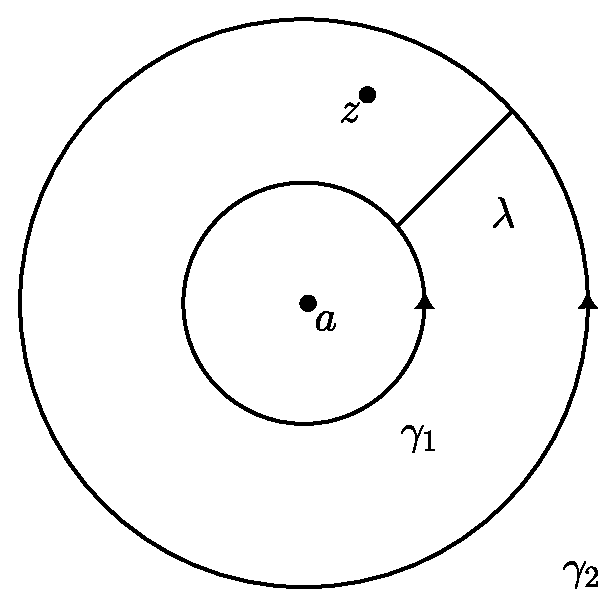
\includegraphics[scale=0.5]{Figures/Chapter5/laurent_series.eps}
        \caption{}
        \label{figure_5.2}
    \end{figure}

    Now, if $R_1<|z-a|<R_2$, choose $r_1$ and $r_2$ such that
    $R_1<r_1<|z-a|<r_2<R_2$, and take $\y_1(t)=a+r_1e^{it}$ and
    $\y_2(t)=a+r_2e^{it}$, on $0 \leq t \leq 2\pi$ (see figure
    \ref{figure_5.2}). Choose, also, a straight radial line segment $\l$ from a
    point on $\y_1$ to a point on $\y_2$, such that $z \notin \{\l\}$. Now,
    notice that $\y_1$ and $\y_2$ are homotopic in the annulus $A$, so we have a
    closed rectifiable path  $\y_1-\y_2-\l$ which is nullhomotopic. Moreover, we
    have $W(\y_2,z)=1$ and $W(\y_1,z)=0$. Thus, using Cauchy's integral formula
    gives
    \begin{equation*}
        f(z)=\frac{1}{2i\pi}\int_{\y}{\frac{f(w)}{(w-z)} \ dw}=f_1(z)+f_2(z)
    \end{equation*}
    Now, since both $f_1$ and $f_2$ are analytic, we can expand them into their
    power series, that is, we have
    \begin{equation*}
        f_2(z)=\sum_{n=0}^\infty{a_n(z-a)^n} \text{ and }
        f_1(z)=\sum_{n=0}^\infty{b_n(z-a)^n}
    \end{equation*}
    Now, define $g$ on  $0<|z|<\frac{1}{R_1}$ by
    \begin{equation*}
        g(z)=f_1(a+\frac{1}{z})
    \end{equation*}
    so that the point $z=0$ is an isolated singularity. If  $r>R_1$, lettign
    $\p(z)=d(z,C)$, where $C=\{w \in \C : |w-a|=r\}$, and taking $M=\max_{w \in
    C}{\{|f(w)|\}}$. Then for all $|z-a|>r$, we have
    \begin{equation*}
        |f_1(z)| \leq \frac{Mr}{\p(z)}
    \end{equation*}
    Notice however that as $z \xrightarrow{} \infty$, $\p(z) \xrightarrow{}
    \infty$, so that $\lim{g(z)}=0$ as $z \xrightarrow{} 0$. This makes $z=0$ a
    removable singularity of $g$. Defining then  $g(0)=0$, we get that $g$ is
    analytic on the ball  $B(0,\frac{1}{R_1})$ Thus, let
    \begin{equation*}
        g(z)=\sum_{n=0}^\infty{B_nz^n}
    \end{equation*}
    the power series expansion of $g$ about  $z=0$. This give that
    \begin{equation*}
        f_1(z)=\sum_{n=1}^\infty{a_{-n}(z-a)^{-n}}
    \end{equation*}
    Moreover, this series converges absolutely and uniformly on small enough
    annuli, so that we obtain uniqueness of the series. Moreover, we get that
    \begin{equation*}
        a_n=\frac{1}{2i\pi}\int_\y{\frac{f(z)}{(z-a)^{n+1}} \ dz}
    \end{equation*}
\end{proof}
\begin{corollary}
    Let $z=a$ be an isolated singularity of a complex-valued function  $f$, Then
    the following are true.
    \begin{enumerate}
        \item[(1)] $z=a$ is a removable singularity if, and only if  $a_n=0$ for
            all  $n \leq -1$.

        \item[(2)] $z=a$ is a pole of order  $m$ if, and only if  $a_{-m} \neq
            0$, and $a_n=0$ for all  $n \leq -(m+1)$.

        \item[(3)] $z=a$ is an essential singularity if, and only if $a_n \neq 0$
            for infinitely many negative integers  $n \in \Z^-$.
    \end{enumerate}
\end{corollary}

\begin{theorem}[The Casorati-Weierstrass Theorem]\label{5.1.4}
    If $f$ is an analytic function with an essential singularity at $z=a$,
    then for all  $\d>0$, the closure
    \begin{equation*}
        \cl{f(A_\d)}=\C
    \end{equation*}
    where $A_\d=\{z \in \C : 0<|z-a|<\d\}$.
\end{theorem}
\begin{proof}
    Let $f$ be analytic on the annulus $A_R=\{z \in \C : 0<|z-a|<R\}$. Suppose
    that for all $c \in \C$, there is an $\e>0$ for which
    \begin{equation*}
        |f(z)-c| \geq \e \text{ whenever } |z-a|<\d \text{ for all } z \in A_R
    \end{equation*}
    Then we get
    \begin{equation*}
        \lim{|z-a|^{-m}|f(z)-c|}=\infty \text{ as } z \xrightarrow{} a
    \end{equation*}
    implying that $(z-a)^{-m}(f(z)-c)$ has a pole of order $m$ at the point
    $z=a$. Then we have
    \begin{equation*}
        \lim{|z-a|^{m+1}|f(z)-c|}=0 \text{ as } z \xrightarrow{} a
    \end{equation*}
    hence
    \begin{equation*}
        |z-a|^{m+1}|f(z)| \leq |z-a|^{m+1}|f(z)-c|+|z-a|^{m+1}|c|
    \end{equation*}
    giving that $|z-a|^{m+1}|f(z)| \xrightarrow{} 0$ as $z \xrightarrow{}
    \infty$. This gives a removable singularity fo $(z-a)^mf(z)$, which
    contradicts tour assumption that $z=a$ is an essential singularity.
\end{proof}
